\begin{figure}[H]
\centering
	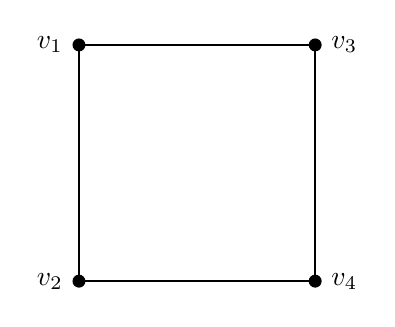
\begin{tikzpicture}
      \tikzset{enclosed/.style={draw, circle, inner sep=0pt, minimum size=.15cm, fill=black}}
%% Vertices
	%ikke orienteret
      	\node[enclosed, label={left, above: $v_1$}] (v1) at (0,3) {};
     	\node[enclosed, label={left, below: $v_2$}] (v2) at (0,0) {};
     	\node[enclosed, label={right, above: $v_3$}] (v3) at (3,3) {};
     	\node[enclosed, label={right, below: $v_4$}] (v4) at (3,0) {};    	
%Edges
	%Ikke orientered
		\path [thick] (v1) edge (v2);
		\path [thick] (v1) edge (v3);
		\path [thick] (v2) edge (v4);
		\path [thick] (v3) edge (v4);

\end{tikzpicture}
	\caption{Simpel graf.}
	\label{fig:laengste.vej}
\end{figure}